% Appendix A

\chapter{Appendices}

\section{A. Further detail of experiments}

\section{Bayesian Inference}

Prior probabilities were calculated or each half-hourly period in a week. Fig \ref{fig10b} shows the calculations for the first 2.5 hours of a Sunday (d-hour-hh format). 

Our parameter of interest is the mean for the Beta distribution representing the probability of play in that time period. We estimate this by calculating probability of a play (total plays in period / count of plays and non-plays) per user, then taking the mean and variance across users. $a$ and $b$ are then determined as:
$a = (\frac{(1- \mu)}{\sigma} - \frac{1}{\mu}) \mu^2$
and
$\beta=\alpha\left(\frac{1}{\mu}-1\right)$.

\begin{figure}[h!]
	\centering
	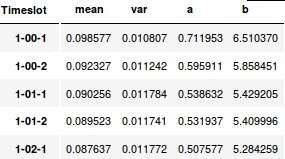
\includegraphics[width=4cm, keepaspectratio,]{fig010b.jpg}
	\caption{}
	\label{fig10b}
\end{figure} 

This allows us to visualize the prior probability for any given time period as shown in \ref{fig10c}.

\begin{figure}[h!]
	\centering
	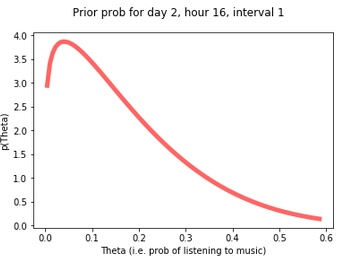
\includegraphics[width=5cm, keepaspectratio,]{fig010c.jpg}
	\caption{}
	\label{fig10c}
\end{figure} 

Once established we can calculate the liklihood of an individual user listening to music in a given time period by passing their observations as they come in for a specific timeslot $s$: $(H_{t,s})$ , into a Beta-Binomial formula to determine the probability of listening at the next occurence of that time slot as shown in <TBC>

Finally the threshold at which we determine that a probability constitutes a Play event is determined by comparing the false positive rates with the true positive rates using a ROC curve (\ref{fig10d}). This tells us that 0.4 is the optimal threshold at which to determine a Play event.

\begin{figure}[h!]
	\centering
	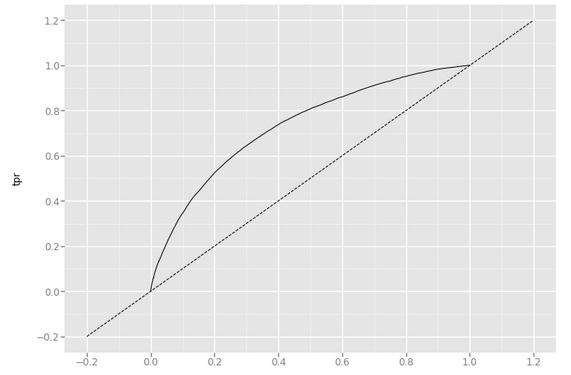
\includegraphics[width=5cm, keepaspectratio,]{fig010d.jpg}
	\caption{ROC curve showing 0.4 as the optimal threshold}
	\label{fig10d}
\end{figure} 

The results from the model are shown in figure \ref{fig10e}. We see that the recall and precision of play events (as denoted by 1) is very low suggesting that relying on a Bayesian approach centered around a weekly profile of each users habits is not an effective method for predicting a play event for a new time period.

\begin{figure}[h!]
	\centering
	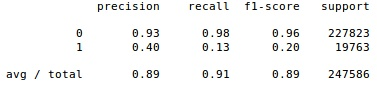
\includegraphics[width=7cm, keepaspectratio,]{fig010e.jpg}
	\caption{Beta-Bionmial Model Results}
	\label{fig10e}
\end{figure} 

\section{Feature analysis}

An advantage of logistic regression over non-linear models is that the coefficients are easily interpretable. While featuer engoneering was not the focus of this research an examination of these can yield insight into which features may be unecessary. 

\begin{figure}[h!]
	\centering
	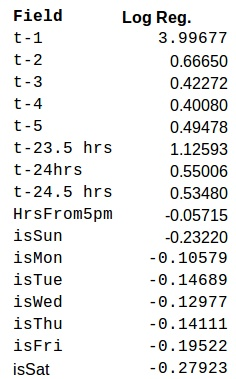
\includegraphics[width=4cm, keepaspectratio,]{fig014.jpg}
	\caption{}
	\label{fig14}
\end{figure} 

Fig \ref{fig14} shows that $t-1$ was by far the most important feature. This is expcted and it's importance crowds out the other features. Interestingly the t-24 hour period appears to have a stronger influence than $t-2$ to $t-5$ once $t-1$ has been accounted for. This reflects the daily patterns we observed in the preliminary analysis. The days of the week also pick up on the fact that weekeneds are somewhat different to weekdays thereby offering one area where the model could be simplified. Finally the hours from 5pm have a very small impact, and is likely unecessary if $t-24hrs$ is also used

\section{RNN Hyper parameter tuning}

For our evaluation of the RNN-LSTM model the dataset was reduced in order to perform the desired number of hyperparameter tests. It was found that the number of hidden layers, units, timeteps, samples, and iterations all played a signficant part in impacting the time it took to train the model. Typical run times were several hours long. 

Fig \ref{fig15} shows the results of some of the other tests that were performed. The improvment in performance comes with an increased in hidden layers, although this also leads to longer training times.

\begin{figure}[h!]
	\centering
	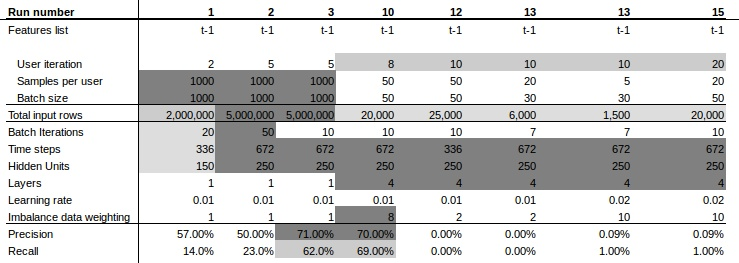
\includegraphics[width=7cm, keepaspectratio,]{fig015.jpg}
	\caption{}
	\label{fig15}
\end{figure}

\section{Adaptability to new users}

We also looked at the performance of models when it comes to learning the patterns of new users. Tie figures below show how the accuracy stablizied over time for each of the 10 test users. The periods indicate half-hourly intervals with 2-3,000 periods (1.5-2 months) appearing to be the time it takses to learn the habits of a typical user. 
\begin{figure}[h!]
	\centering
	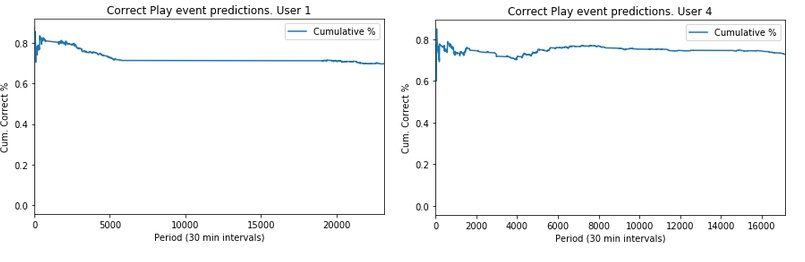
\includegraphics[width=7cm, keepaspectratio,]{fig008a.jpg}
	\caption{}
	\label{fig:fig8a}
\end{figure} 

\begin{figure}[h!]
	\centering
	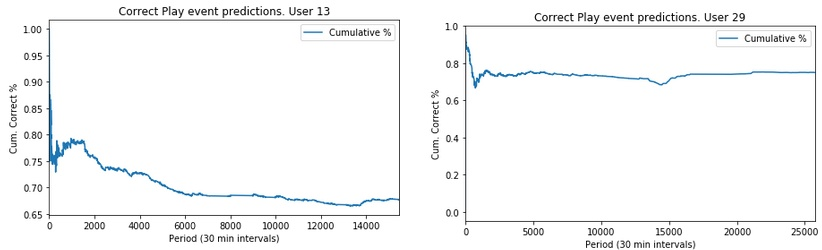
\includegraphics[width=7cm, keepaspectratio,]{fig008b.jpg}
	\caption{}
	\label{fig:fig8b}
\end{figure} 

\begin{figure}[h!]
	\centering
	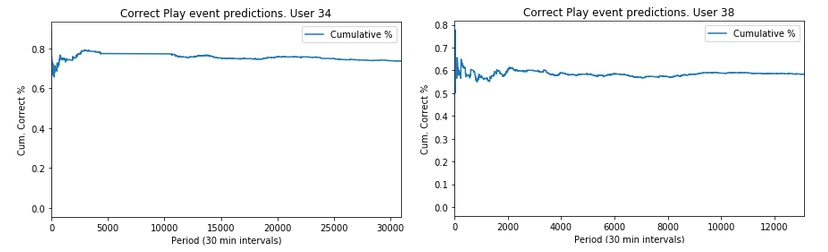
\includegraphics[width=7cm, keepaspectratio,]{fig008c.jpg}
	\caption{}
	\label{fig:fig8c}
\end{figure} 

\begin{figure}[h!]
	\centering
	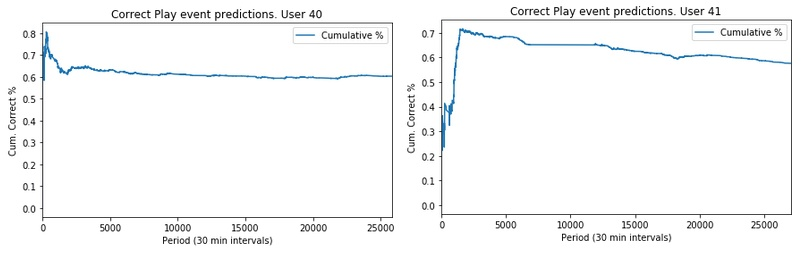
\includegraphics[width=7cm, keepaspectratio,]{fig008d.jpg}
	\caption{}
	\label{fig:fig8d}
\end{figure} 

\begin{figure}[h!]
	\centering
	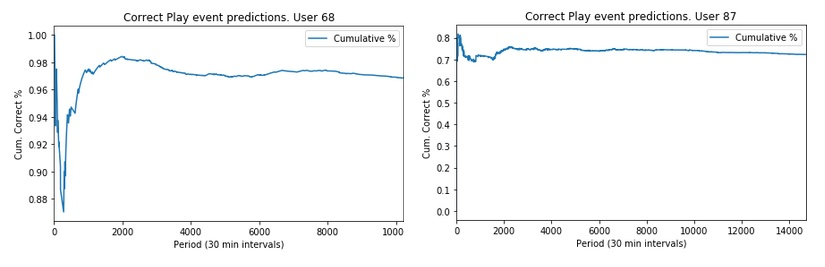
\includegraphics[width=7cm, keepaspectratio,]{fig008e.jpg}
	\caption{}
	\label{fig:fig8e}
\end{figure} 


From these charts it appears that two months worth of data is required to for the model to rget trained up on a new user.


\section{Content not used} % Main appendix title

Intro:
At an aggregate level, behaviour may appear to be deterministic, such as the times at which peak rush-hour occurs, but such behaviour is often composed of thousands or millions of individual stochastic processes such as the decisions made by individuals as to whether to leave work at 5pm or continue working a little longer.

While the modeling of aggregate patterns is well understood, these models ofen breakdown when applied to customizing results for individual users. At this level the temporal patterns of an individual combined with the behaviour of the population may be a better predictor of event timing. For instance, sticking with the example above, the times at which a person has lunch during the day may help predict that they will finish work a little later.

